\chapter{Implementation}\label{ch:implem}

As the previous chapter covered, several different parameters were experimented with, both in preliminary trials and during a more thorough performance testing phase.  These included primarily modifier weight, mutation rate, and crossover rate, all thoroughly trialed with thirty different randomly generated seeds.  As performance test results were acquired and data analyzed, the prominent trend seemed to be that this optimization process succeeded in reducing the negative characteristics used to measure the efficiency of the traffic control network.  To gain this insight, the starting and resulting fitnesses were both recorded and compared to each other to gain some sense of the increase in fitness from either; while some, in fact, had a smaller  increase in fitness, only 10\% while some had 30\% increase in fitness.  Additional preliminary trials were run on larger populations and larger generation numbers and while there appeared to be an increase in performance, due to the time sensitive nature of the project, these parameters were not overly tested due to their lengthy execution time.

In the 2000+ trials that were run, the percent change in fitness was 35.83\% while the minimum was actually 0\% and a mean of 16.1\%.  This is regardless of the different changes however it shows that this system is, in fact, applicable to the problem proposed.  The case where the largest occurred was shown when the fuel consumption had the heaviest weight.  An interesting observation, as exemplified in the graph below is that when the heavier consumption rate, the lower the mutation rate, regardless of the crossover rate.  In fact this trend, as noticed in the other graphs below, is consistent throughout all performance testing.  Values in these graphs closer to 0, other than the percentage change values, indicate a sense of ``better'' optimization.  The only true change in scaling arose when more weight was given to the fuel consumption which was a matter of flooding the units, however even then the trend is still obvious.
\vspace*{-2in}
\begin{figure}[h!]	
	\hspace*{-2in}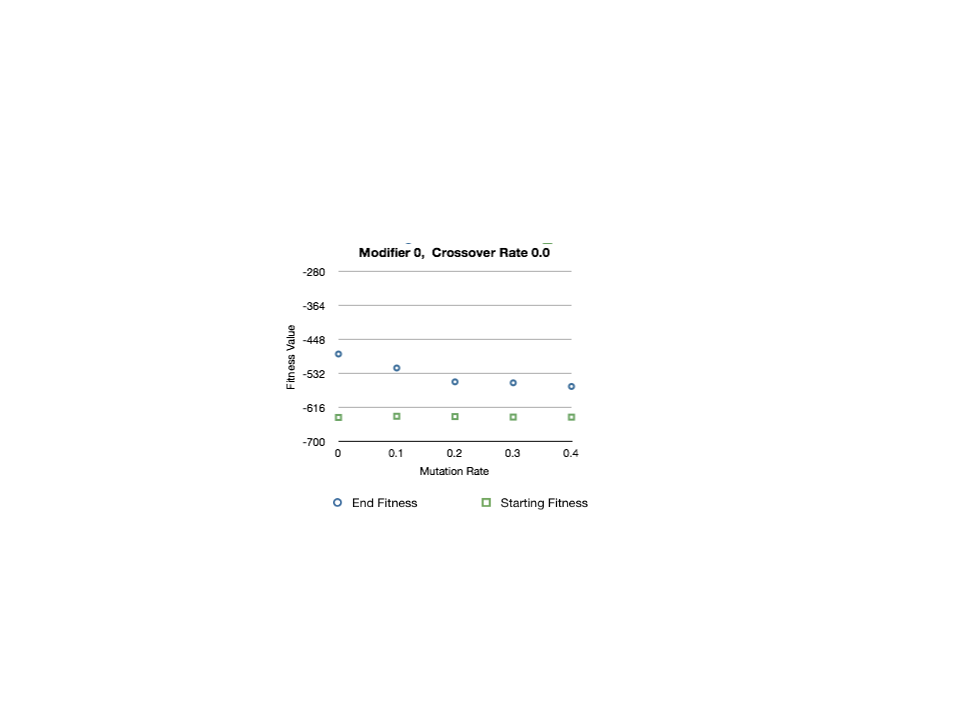
\includegraphics[width=10in]{images/FitMute00.png}\hspace*{0in}\vspace*{-2in}
	\caption{Equally weighted variables, 0.0 crossover rate fitness comparisons}
	\label{Figure 1}
\end{figure}\vspace*{-4in}


\begin{figure}[h!]
	\hspace*{-2in}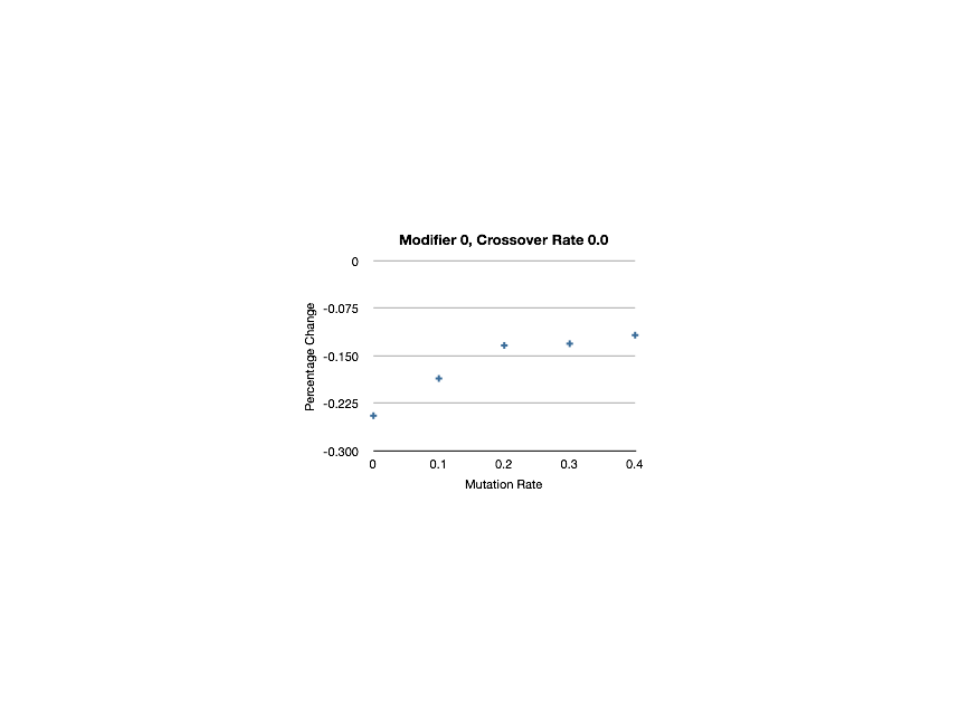
\includegraphics[width=10in]{images/FitMute00Percent.png}\hspace*{0in}\vspace*{-2in}
	\caption{Percent change between starting fitnesses and final fitnesses}
	\label{Figure 2}
\end{figure}

\newpage
It should be noted that values closer to 0 indicate a ``better" fitness level and closer to optimization, while percentage change values further from 0 indicate that a greater change happened between original fitness to final fitness.  Additionally, all of these graphs use average values of the twenty different seeds used for each trial.  This was to ensure an accurate coverage and number of repetitions were done.
\vspace*{-2in}
\begin{figure}[h!]	
	\hspace*{-2in}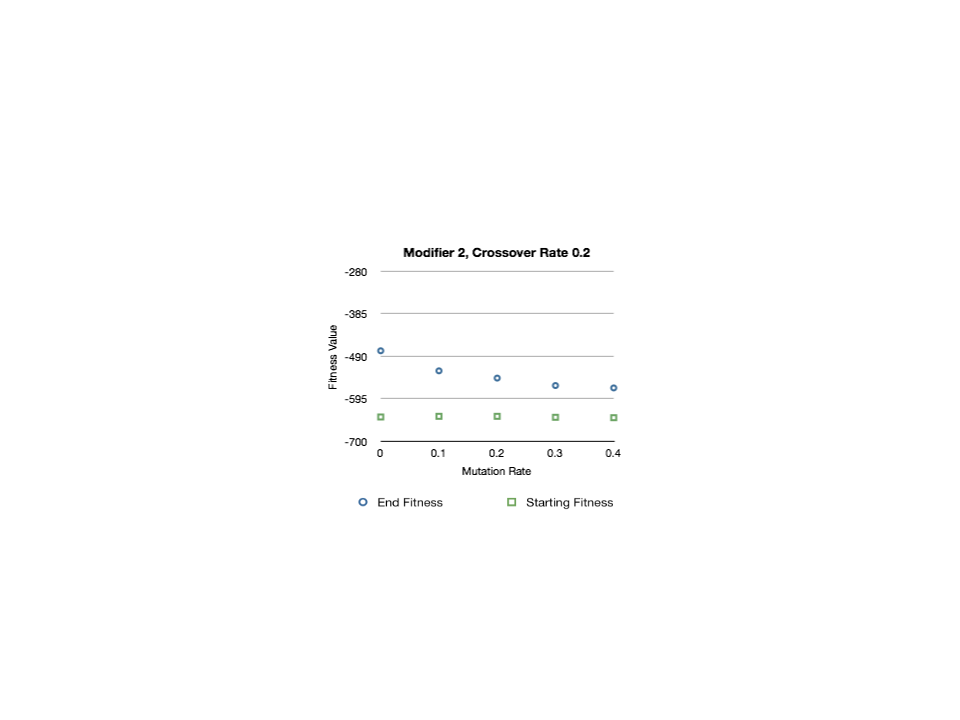
\includegraphics[width=10in]{images/FitMute02.png}\hspace*{0in}\vspace*{-2in}
	\caption{Time delay heavily weighted (.6 vs .3), 0.2 crossover rate fitness comparisons}
	\label{Figure 3}
\end{figure}

\begin{figure}[h!]	
	\hspace*{-2in}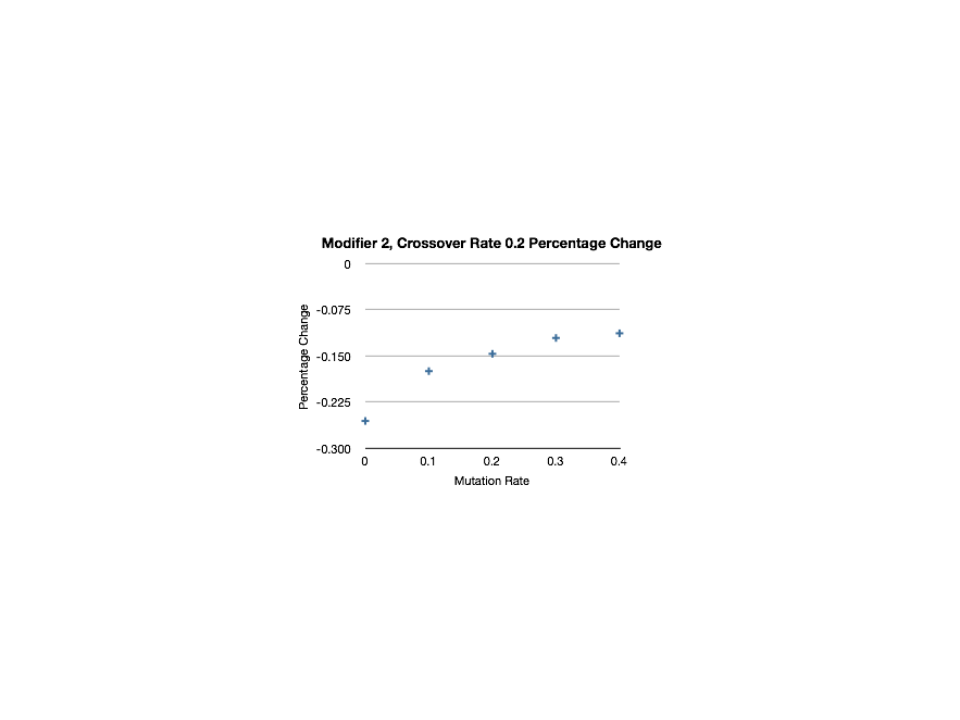
\includegraphics[width=10in]{images/FitMut02Percent.png}\hspace*{0in}\vspace*{-2in}
	\caption{Percent change between starting fitnesses and final fitnesses}
	\label{Figure 4}
\end{figure}

\begin{figure}[h!]
	\hspace*{-2in}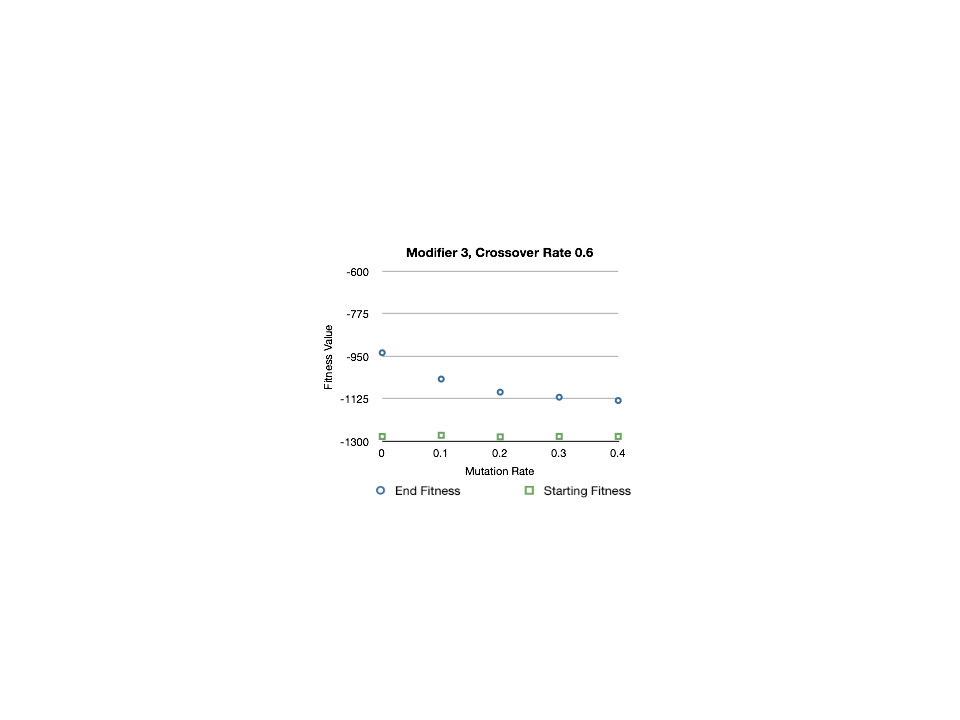
\includegraphics[width=10in]{images/FitMut03.png}\hspace*{0in}\vspace*{-2in}
	\caption{Fuel consumption heavily weighted (.6 vs .3), 0.6 crossover rate}
	\label{Figure 5}
\end{figure}

\begin{figure}[h!]
	\hspace*{-2in}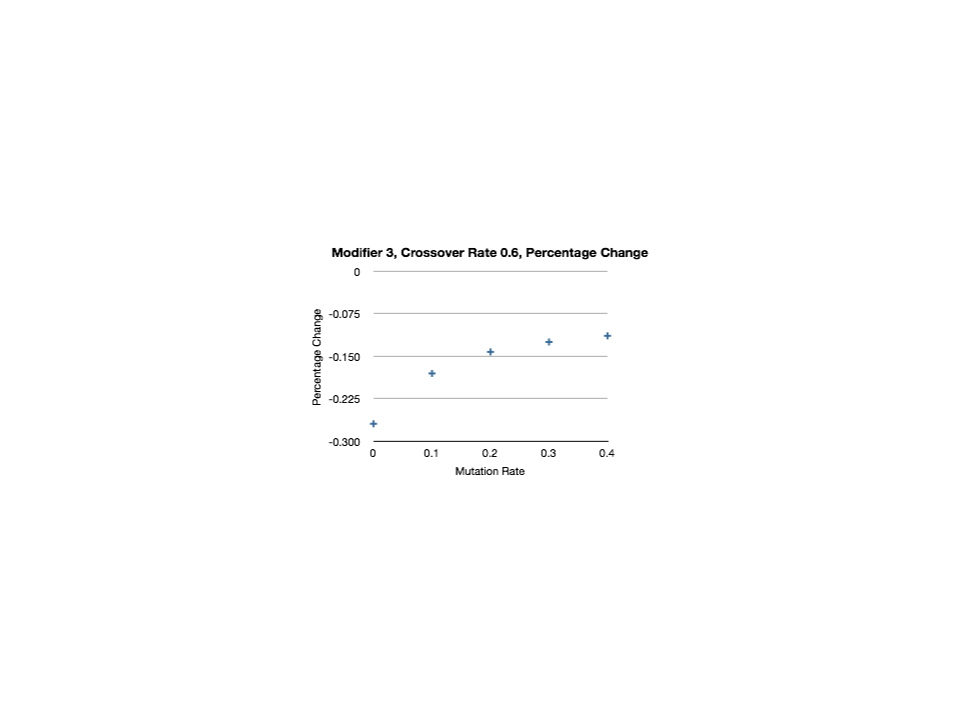
\includegraphics[width=10in]{images/FitMut03Per.png}\hspace*{0in}\vspace*{-2in}
	\caption{Percent change between starting fitnesses and final fitnesses}
	\label{Figure 6}
\end{figure}
\newpage
The precise values of the trials are as follows.  Generation number was held constant at 25 generations per trial, and population size was held at 20 individuals per generation.  Crossover probability ranged from 0.0 to 0.6, incrementing by 0.2 each iteration.  Mutation rate ranged from 0.0 to 0.5 incrementing by 0.1 each iteration.  Additionally there were four modifiers used to adjust the weight of the different criteria of the fitness function.  The weights are either all even with a multiplier value of 0.33, or one is weighted more heavily as 0.66 while the others remain 0.33.  Modifier 0 represents an even weighting, modifier 1 weighs time transit more heavily, modifier 2 weighs time delay more heavily, and finally modifier 3 weighs gas usage more heavily.  These do not seem to disrupt trend but rather appear to influence the scaling as shown in there graphs.

These results support the hypothesis that using genetic algorithms can a good metric and standard for optimizing these kind of idealized city plan systems.  This entails that genetic algorithms, or this approach to using genetic algorithms, may be appropriate to select, firstly, whether or not an intersection has a stop sign or a traffic light at each node, and secondly, the timings at each of these intersections.  This means that even though there are a myriad of variables and possible configurations, the evolutionary approach of genetic algorithms allows for the program to approach a local or global ideal state.  This is not to say that the chosen pipelines and manners in which selection and crossover were performed, could not have been improved.  For this study, the simplest of genetic algorithms was implemented using, as seen in the parameters file earlier, tournament selection, two sources for breeding, and a tournament size of two, meaning that from each generation, four random individuals were selected, and the two best of these four were used as parents for the next generation.  There are several alternatives to many of these pipelines that were used and perhaps in future studies, these may prove to perform better for this type of problem.  